\documentclass{beamer}
\usepackage{hyperref, mathrsfs, picture, tabto, tikz, ulem}
\usecolortheme[RGB={34, 139, 34}]{structure}
\usetheme{Singapore}
\setbeamertemplate{navigation symbols}{\insertframenumber}
\definecolor{dodgerblue}{rgb}{0.12, 0.56, 1.0}
\definecolor{darkorange}{rgb}{1.0, 0.55, 0.0}
\definecolor{forestgreen}{rgb}{0.13, 0.55, 0.13}

\def\A{\mathcal A}\def\B{\mathcal B}\def\C{\mathcal C}\def\D{\mathcal D}
\def\E{\mathcal E}\def\F{\mathcal F}\def\G{\mathcal G}\def\J{\mathcal J}
\def\L{\mathcal L}\def\M{\mathcal M}\def\N{\mathcal N}\def\O{\mathcal O}
\def\P{\mathcal P}\def\Q{\mathcal Q}\def\R{\mathcal R}\def\S{\mathcal S}
\def\T{\mathcal T}\def\W{\mathcal W}\def\V{\mathcal V}\def\X{\mathcal X}
\def\Y{\mathcal Y}\def\Z{\mathcal Z}
\def\mE{\mathbb E}\def\mN{\mathbb N}\def\mP{\mathbb P}\def\mR{\mathbb R}
\def\mS{\mathbb S}
\def\bE{{\bf E}}
\def\bx{{\bf x}}
\def\prob{\mbox{\bf prob}}\def\tr{\mbox{\bf tr}}
\def\l{\left}\def\r{\right}\def\lf{\lfloor}\def\rf{\rfloor}
\def\un{\underline}
\def\theat{\theta}\def\lambad{\lambda}\def\lamda{\lambda}
\def\iid{\stackrel{\mbox{\scriptsize i.i.d.}}{\sim}}
\def\ind{\stackrel{\mbox{\scriptsize ind.}}{\sim}}
\def\minimize{\mbox{minimize}\hspace{4mm}}
\def\maximize{\mbox{maximize}\hspace{4mm}}
\def\subjectto{\mbox{subject to}\hspace{4mm}}

\title{True wOBA:\\
    \small Estimation of true talent level for batters}
\author{Scott Powers and Eli Shayer}
\institute{Stanford University}
\date{2016 SABR Analytics Conference}
\begin{document}

\begin{frame}
\titlepage
\hfill
\includegraphics[width = 1in]{../figs/ssac.png}
\end{frame}

\begin{frame}{Review: regression to the mean}
\begin{tabular}{ccc}
True strikeout probability  & $p$ & {\color{white}?}\\
    \vspace{2mm}\\
Observed strikeout rate     & $\hat p = \frac{\mbox{\tt K}}{\mbox{\tt PA}}$
    & {\color{white}$\frac{23}{138} = 16.7\%$}\\
    \vspace{2mm}\\
Regression to the mean      & $p^* = \frac{\mbox{\tt K} + N\bar p}
    {\mbox{\tt PA} + N}$ &
    {\color{white}$\frac{23 + 40(20.4\%)}{138 + 40} = 17.5\%$}
\end{tabular}\\
\vspace{4mm}
\begin{columns}
\begin{column}{0.6\textwidth}
\hfill {\small $\bar p =$ league average strikeout rate}\\
\vspace{1cm}
$${\color{white} N = \frac{\bar p(1 - \bar p)}{\sigma^2_T}}$$
\end{column}
\begin{column}{0.4\textwidth}
\centering
\includegraphics[width = 3cm]{../figs/gosewhite.png}\\
\large {\color{white} Tuffy Gosewisch}\\
{\color{white}\tiny Ralph Freso, Getty Images}
\end{column}
\end{columns}
\end{frame}

\begin{frame}{Review: regression to the mean}
\begin{tabular}{ccc}
True strikeout probability  & $p$ & ?\\
    \vspace{2mm}\\
Observed strikeout rate     & $\hat p = \frac{\mbox{\tt K}}{\mbox{\tt PA}}$
    & $\frac{23}{138} = 16.7\%$\\
    \vspace{2mm}\\
Regression to the mean      & $p^* = \frac{\mbox{\tt K} + N\bar p}
    {\mbox{\tt PA} + N}$ & $\frac{23 + 40(20.4\%)}{138 + 40} = 17.5\%$
\end{tabular}\\
\vspace{4mm}
\begin{columns}
\begin{column}{0.6\textwidth}
\hfill {\small $\bar p =$ league average strikeout rate}\\
\vspace{1cm}
$${\color{white} N = \frac{\bar p(1 - \bar p)}{\sigma^2_T}}$$
\end{column}
\begin{column}{0.4\textwidth}
\centering
\includegraphics[width = 3cm]{../figs/gosewisch.png}\\
\large Tuffy Gosewisch\\
{\color{gray}\tiny Ralph Freso, Getty Images}
\end{column}
\end{columns}
\end{frame}

\begin{frame}{Review: regression to the mean}
\begin{tabular}{ccc}
True strikeout probability  & $p$ & ?\\
    \vspace{2mm}\\
Observed strikeout rate     & $\hat p = \frac{\mbox{\tt K}}{\mbox{\tt PA}}$
    & $\frac{23}{138} = 16.7\%$\\
    \vspace{2mm}\\
Regression to the mean      & $p^* = \frac{\mbox{\tt K} + N\bar p}
    {\mbox{\tt PA} + N}$ & $\frac{23 + 40(20.4\%)}{138 + 40} = 17.5\%$
\end{tabular}\\
\vspace{4mm}
\begin{columns}
\begin{column}{0.6\textwidth}
\hfill {\small $\bar p =$ league average strikeout rate}\\
\vspace{1cm}
$$N = \frac{\bar p(1 - \bar p)}{\sigma^2_T}$$
\end{column}
\begin{column}{0.4\textwidth}
\centering
\includegraphics[width = 3cm]{../figs/gosewisch.png}\\
\large Tuffy Gosewisch\\
{\color{gray}\tiny Ralph Freso, Getty Images}
\end{column}
\end{columns}
\end{frame}

\begin{frame}{Review: regression to the mean}
$$p \sim \N(\bar p, \sigma^2_T) \hspace{1cm}
{\color{white} \hat p|p \sim \N\l(p,~\sigma^2_L = \frac{p(1-p)}{n}\r)}$$
\begin{center}
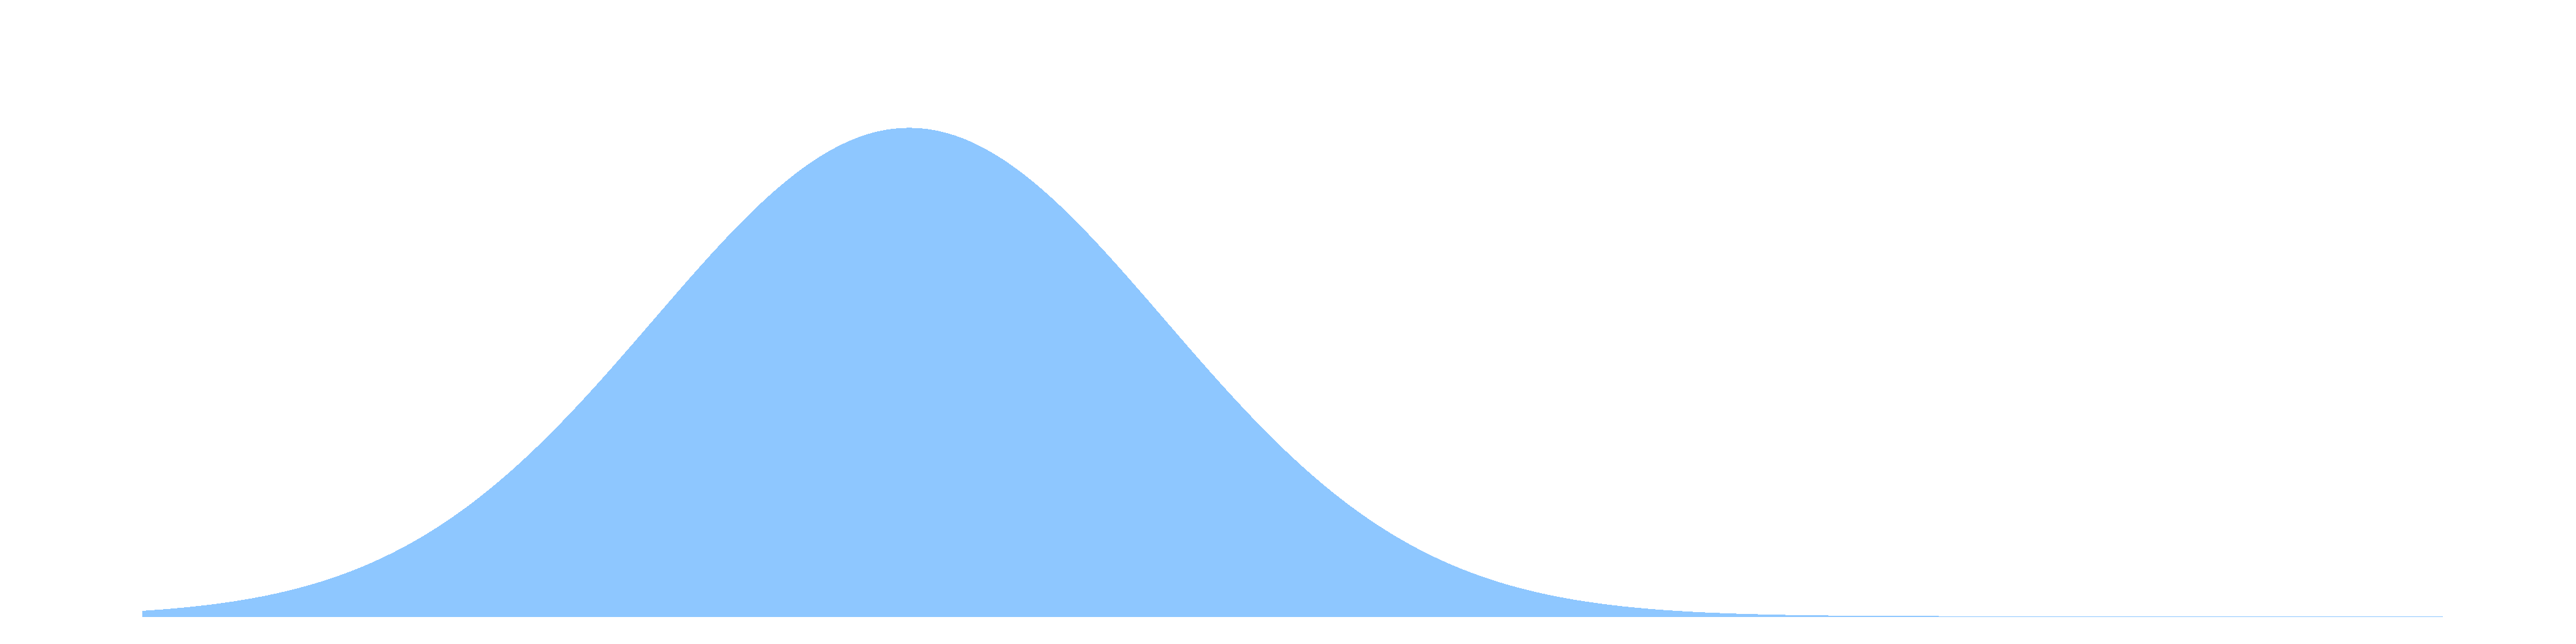
\includegraphics[width = \textwidth]{../figs/talent.pdf}\\
\end{center}
\vspace{-6mm}\tabto*{37mm}$\uparrow$\\
\tabto*{37mm}$\bar p$
{\color{white}
\vspace{-5mm}\tabto*{58mm}$\uparrow$\\
\tabto*{57.5mm}$\hat p$
\vspace{-4.5mm}\tabto*{44mm}$\uparrow$\\
\tabto*{44mm}$p^*$\\}
$${\color{white} p^* = E[p|\hat p] = \arg\min_{p^*}{E[(p - p^*)^2|\hat p]}
    = \frac{\sigma_T^{-2}\bar p + \sigma_L^{-2}\hat p}
    {\sigma_T^{-2} + \sigma_L^{-2}}}$$
\end{frame}

\begin{frame}{Review: regression to the mean}
$$p \sim \N(\bar p, \sigma^2_T) \hspace{1cm}
\hat p|p \sim \N\l(p,~\sigma^2_L = \frac{p(1-p)}{n}\r)$$
\begin{center}
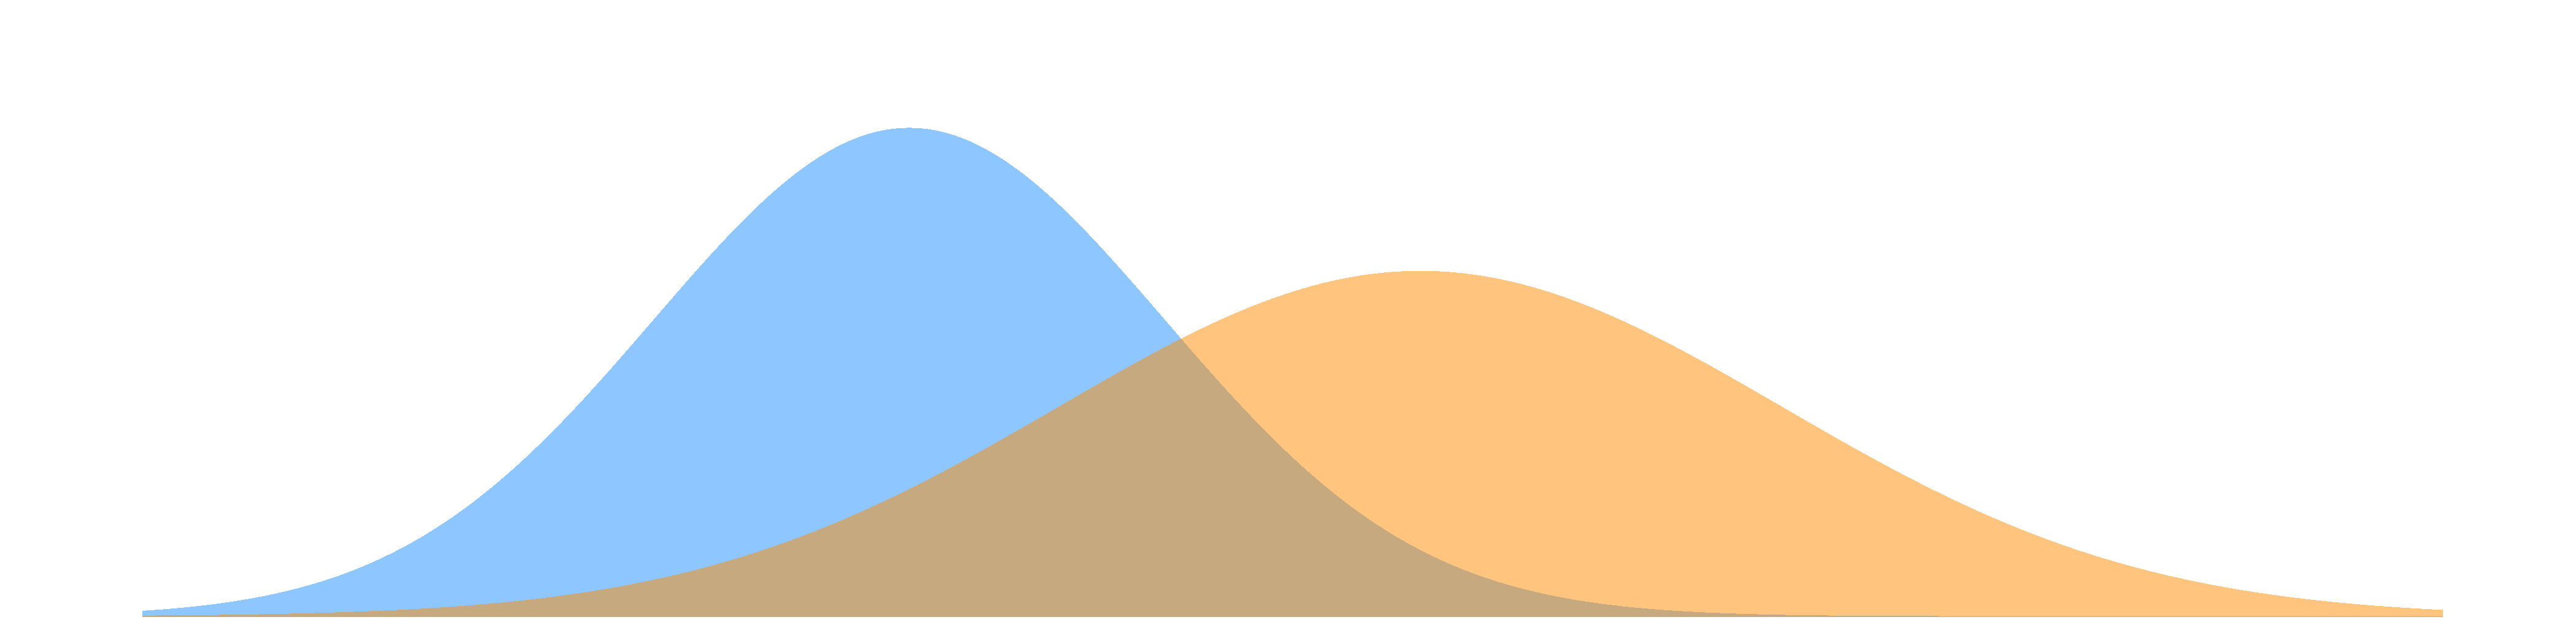
\includegraphics[width = \textwidth]{../figs/talent-skill.pdf}
\end{center}
\vspace{-6mm}\tabto*{37mm}$\uparrow$\\
\tabto*{37mm}$\bar p$
\vspace{-5mm}\tabto*{58mm}$\uparrow$\\
\tabto*{57.5mm}$\hat p$
{\color{white}
\vspace{-4.5mm}\tabto*{44mm}$\uparrow$\\
\tabto*{44mm}$p^*$\\}
$${\color{white} p^* = E[p|\hat p] = \arg\min_{p^*}{E[(p - p^*)^2|\hat p]}
    = \frac{\sigma_T^{-2}\bar p + \sigma_L^{-2}\hat p}
    {\sigma_T^{-2} + \sigma_L^{-2}}}$$
\end{frame}

\begin{frame}{Review: regression to the mean}
$$p \sim \N(\bar p, \sigma^2_T) \hspace{1cm}
\hat p|p \sim \N\l(p,~\sigma^2_L = \frac{p(1-p)}{n}\r)$$
\begin{center}
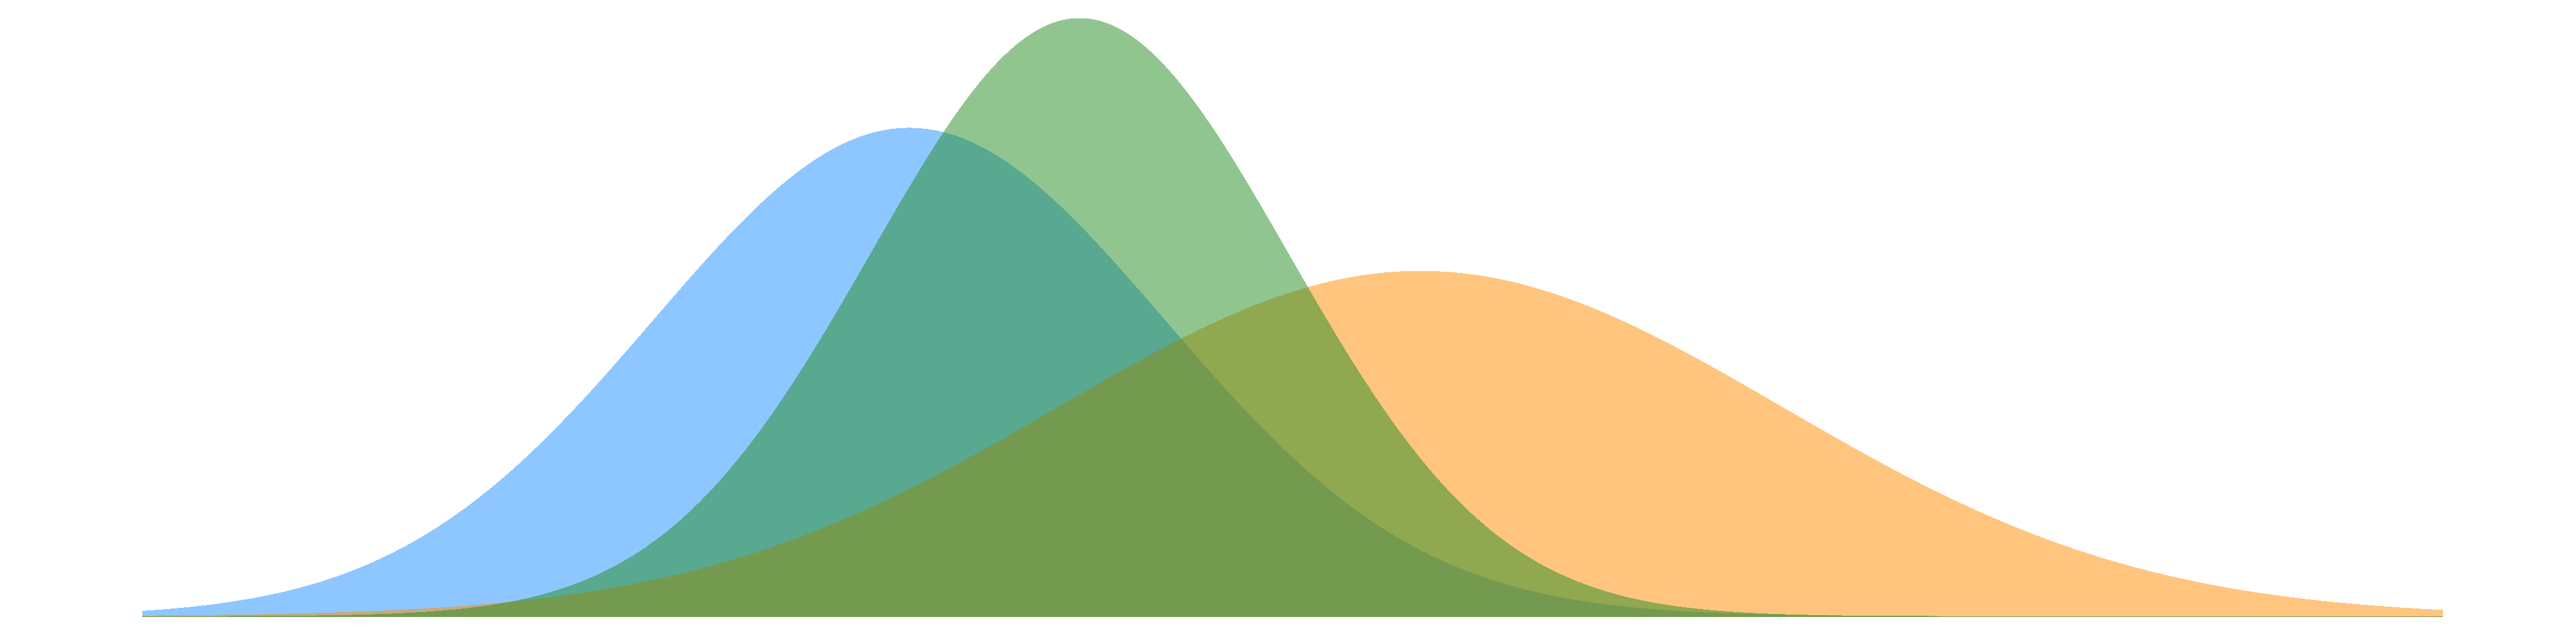
\includegraphics[width = \textwidth]{../figs/talent-skill-post.pdf}
\end{center}
\vspace{-6mm}\tabto*{37mm}$\uparrow$\\
\tabto*{37mm}$\bar p$
\vspace{-5mm}\tabto*{58mm}$\uparrow$\\
\tabto*{57.5mm}$\hat p$
\vspace{-4.5mm}\tabto*{44mm}$\uparrow$\\
\tabto*{44mm}$p^*$\\
$$p^* = E[p|\hat p] = \arg\min_{p^*}{E[(p - p^*)^2|\hat p]}
    = \frac{\sigma_T^{-2}\bar p + \sigma_L^{-2}\hat p}
    {\sigma_T^{-2} + \sigma_L^{-2}}$$
\end{frame}

\begin{frame}{Outline for this presentation}
\begin{itemize}
    \item Theory
    \tabto*{8cm}\makebox(0,0){\put(0, -5.5\normalbaselineskip){$\left.
        \rule{0pt}{2.5\normalbaselineskip}\right\}$ Scott}}
    \begin{itemize}
        \item \sout{Regression to the mean}
        \item Regularized linear regression
        \item Regularization vs. regression to the mean
        \item Regularization vs. mixed effect modelling
    \end{itemize}
    \item Application
    \tabto*{8cm}\makebox(0,0){\put(0, -6\normalbaselineskip){$\left.
        \rule{0pt}{2.6\normalbaselineskip}\right\}$ Eli}}
    \begin{itemize}
        \item Regressing wOBA to the mean
        \item Comparison of true talent estimators
        \item True wOBA results
    \end{itemize}
    \item Discussion
\end{itemize}
\end{frame}

\begin{frame}{A simple linear model}
~{\bf Data}:\\
For plate appearance $i \in \{1, ..., n\}$,\\~\\
$K_i = \l\{\begin{array}{l}1\mbox{ if $i^{th}$ PA results in strikeout}\\
    0\mbox{ otherwise}\end{array}\r.$\\~\\
$B_i =$ identity of batter in $i^{th}$ PA (e.g. Paul Goldschmidt)\\~\\
~{\bf Model}:
$$K_i = \alpha + \beta_{B_i} + \epsilon_i, \hspace{4mm}
    \mbox{where}\hspace{4mm} \epsilon_i \iid \N(0,\sigma^2)$$
~{\bf Estimator}:
$$(\hat\alpha, \hat\beta) = \arg\min\sum_{i=1}^n(K_i - \alpha - \beta_{B_i})^2
    \hspace{4mm} \Rightarrow \hspace{4mm}
    \hat\alpha + \hat\beta_{B} = \frac{\sum_{i:B_i=B}K_i}{\sum_{i:B_i=B}1}$$
\end{frame}

\begin{frame}{Regularized linear regression}
\vspace{-1cm}
\begin{align*}
\mbox{Instead of solving}&\\   (\hat\alpha, \hat\beta) = & \hspace{1mm}
    \arg\min\sum_{i=1}^n(K_i - \alpha - \beta_{B_i})^2,\\
\mbox{let's try solving}&\\    (\alpha^*, \beta^*) = & \hspace{1mm}
    \arg\min\sum_{i=1}^n(K_i-\alpha-\beta_{B_i})^2 + \lambda\sum_B\beta_B^2,
    \hspace{4mm}\lambda > 0.
\end{align*}
The result is
$$\beta^*_B = \frac{\lambda\cdot0 + n_B\hat\beta_B}{\lambda + n_B},\hspace{4mm}
    \mbox{where}\hspace{4mm}n_B = \sum_{i:B_i=B}1$$
\end{frame}

\begin{frame}{Regularization vs. regression to the mean}
Regression to the mean:
$$p^* = \frac{\sigma_T^{-2}\bar p + \sigma_L^{-2}\hat p}
    {\sigma_T^{-2} + \sigma_L^{-2}}$$
{\color{white} -- $\sigma_T^2$ estimated by comparing across-player variance to
    $\sigma^2_L$}\\~\\
Regularization:
$$\alpha^* + \beta^* = \frac{\lambda\hat\alpha + n(\hat\alpha + \hat\beta)}
    {\lambda + B} = \frac{\lambda\bar p + n\hat p}{\lambda + n}$$
{\color{white} -- $\lambda$ chosen by cross-validation}\\~\\
If $\lambda = n\sigma^2_L/\sigma^2_T$, these estimates are identical!
\end{frame}

\begin{frame}{Regularization vs. regression to the mean}
Regression to the mean:
$$p^* = \frac{\sigma_T^{-2}\bar p + \sigma_L^{-2}\hat p}
    {\sigma_T^{-2} + \sigma_L^{-2}}$$
-- $\sigma_T^2$ estimated by comparing across-player variance to
    $\sigma^2_L$\\~\\
Regularization:
$$\alpha^* + \beta^* = \frac{\lambda\hat\alpha + n(\hat\alpha + \hat\beta)}
    {\lambda + B} = \frac{\lambda\bar p + n\hat p}{\lambda + n}$$
{\color{white} -- $\lambda$ chosen by cross-validation}\\~\\
If $\lambda = n\sigma^2_L/\sigma^2_T$, these estimates are identical!
\end{frame}

\begin{frame}{Regularization vs. regression to the mean}
Regression to the mean:
$$p^* = \frac{\sigma_T^{-2}\bar p + \sigma_L^{-2}\hat p}
    {\sigma_T^{-2} + \sigma_L^{-2}}$$
-- $\sigma_T^2$ estimated by comparing across-player variance to
    $\sigma^2_L$\\~\\
Regularization:
$$\alpha^* + \beta^* = \frac{\lambda\hat\alpha + n(\hat\alpha + \hat\beta)}
    {\lambda + B} = \frac{\lambda\bar p + n\hat p}{\lambda + n}$$
-- $\lambda$ chosen by cross-validation\\~\\
If $\lambda = n\sigma^2_L/\sigma^2_T$, these estimates are identical!
\end{frame}

\begin{frame}{Logistic regression}
~{\bf A better model}:
$$\eta_i = \alpha + \beta_{B_i}, \hspace{4mm}\mbox{and}\hspace{4mm}
\mP(K_i = 1|\eta_i) = e^{\eta_i}/(1+e^{\eta_i})$$
\begin{center}
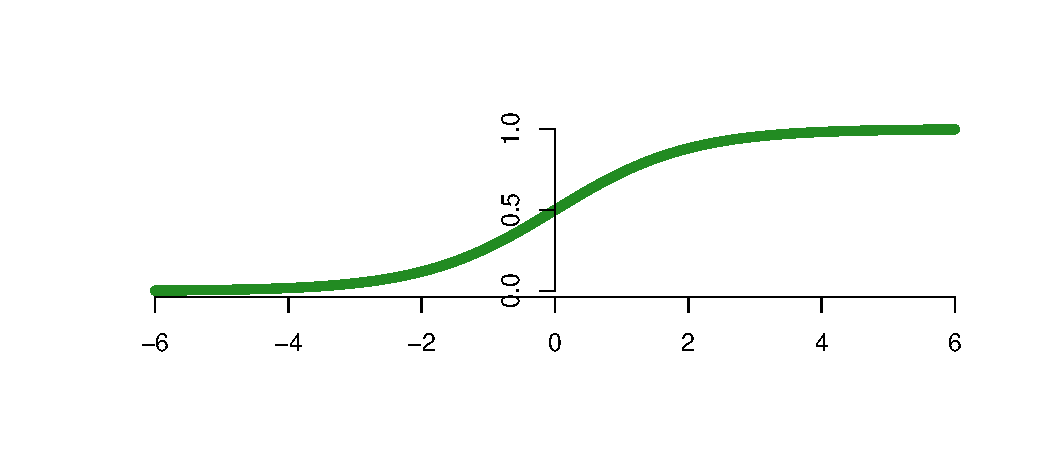
\includegraphics[width = 0.6\textwidth]{../figs/logistic.pdf}
\end{center}
~{\bf Estimator (Ridge)}:
$$(\alpha^*, \beta^*) = \arg\min-\sum_{i=1}^n\log\mP(K_i|\eta_i) +
    \lambda\sum_B\beta_B^2$$
\end{frame}

\begin{frame}{True wOBA}
~{\bf Data}:\\
$Y_i \in \Y = \{\mbox{G, F, K, BB, HBP, 1B, 2B, 3B, HR}\}$\\
$B_i =$ identity of {\bf B}atter in $i^{th}$ PA (e.g. Paul Goldschmidt)\\
$P_i =$ identity of {\bf P}itcher in $i^{th}$ PA (e.g. Zach Greinke)\\
$S_i =$ identity of {\bf S}tadium in $i^{th}$ PA (e.g. Chase Field)\\
$H_i =$ 1 if $B_i$ is on {\bf H}ome team, 0 otherwise\\
$O_i =$ 1 if $B_i$ and $P_i$ have {\bf O}pposite handedness, 0 otherwise\\~\\
~{\bf Model (multinomial logistic regression)}:
$$\eta_{ik} = \alpha_k + \beta_{B_ik} + \gamma_{P_ik} +
    \delta_{S_ik} + \zeta_kH_i + \theta_kO_i$$
$$\mP(Y_i=k|\eta_i) = \frac{e^{\eta_{ik}}}{\sum_{\ell\in\Y}e^{\eta_{i\ell}}}$$
\end{frame}

\begin{frame}{True wOBA}
~{\bf Estimation}:
\begin{align*}
\min&\l\{-\sum_{i=1}^n\mP(Y_i|\eta_i)\r.\\
    &\hspace{4mm} + \l.\sum_{k\in\Y}\lambda_k\l(\sum_B\beta_{Bk}^2
    + \sum_P\gamma_{Pk}^2 + \sum_S\delta_{Sk}^2 + \zeta_k^2 + \theta_k^2\r)\r\}
\end{align*}
\begin{itemize}
    \item Choose $\lambda_k$ via cross validation
    \item For batter $B$, estimated K rate in average situation is
    $$\mP_B(K) = \frac{e^{\alpha^*_K + \beta^*_{BK} + \frac12\zeta^*_K +
    \frac12\theta^*_K}}{\sum_{\ell\in\Y}e^{\alpha^*_\ell + \beta^*_{B\ell} +
    \frac12\zeta^*_\ell + \frac12\theta^*_\ell}}$$
    \item Combine rates of outcomes into True wOBA estimate
\end{itemize}
\end{frame}

\begin{frame}{Random effect model}
~{\bf Model}:
$$\eta_i = \alpha + \beta_{B_i}, \hspace{4mm}\mbox{where}\hspace{4mm}
\beta_B \iid \N(0, \sigma^2_\beta)$$
$$\mP(K_i = 1|\eta_i) = \Phi(\eta_i) \leftarrow \mbox{Normal CDF}$$
\begin{center}
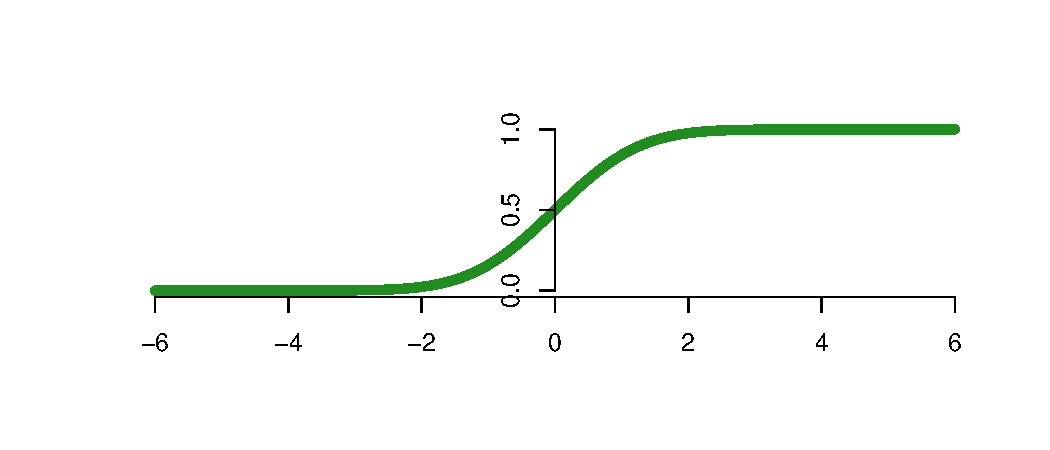
\includegraphics[width = 0.6\textwidth]{../figs/normalcdf.pdf}
\end{center}
~{\bf Estimator (Random)}:
$$(\alpha^*, \beta^*, \sigma^{2*}_\beta) =
    \arg\max L(\alpha, \beta, \sigma^2_\beta|B_i, K_i)$$
\end{frame}

\begin{frame}
\centering\Huge Application
\end{frame}

\begin{frame}
\centering\LARGE Regression to the Mean
\end{frame}

\begin{frame}{Regression to the mean for each outcome probability}
For each outcome, use $1^{st}$ 200 PAs to predict rate on next 200 PAs\\~\\
\centering
\begin{tabular}{c|r|cc}
\multicolumn{2}{c}{}    & (Naive)           & (Regressed)\\
    & $\hat\sigma^2_T$  & RMSE($\hat p$)    & RMSE($p^*$)\\
    \hline
G   & 15.85             & 4.80              & 4.42\\
F   & 20.13             & 4.45              & 4.22\\
K   & 29.10             & 4.19              & 3.89\\
BB  &  6.26             & 3.33              & 3.04\\
HBP &  0.24             & 0.94              & 0.80\\
1B  &  7.02             & 3.81              & 3.17\\
2B  &  0.45             & 2.01              & 1.62\\
3B  &  0.13             & 0.74              & 0.67\\
HR  &  1.88             & 1.79              & 1.61
\end{tabular}\\
{\scriptsize Units: percentage points}\\
{\bf Upshot}: Different population variances for different outcomes,\\
but regression to the mean improves RMSE for all of them!
\end{frame}

\begin{frame}{Regressed wOBA vs. observed wOBA}
\centering
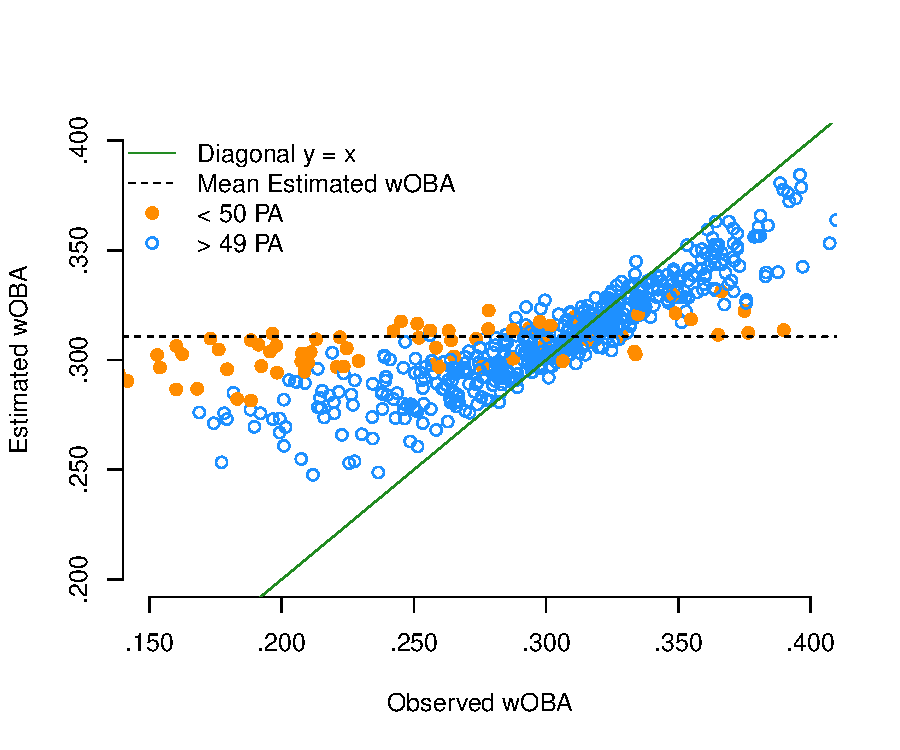
\includegraphics[width = 0.8\textwidth]
    {../figs/woba-observed-v-estimated-slides.pdf}
\end{frame}

\begin{frame}{Projected change in wOBA vs. BABIP}
\centering
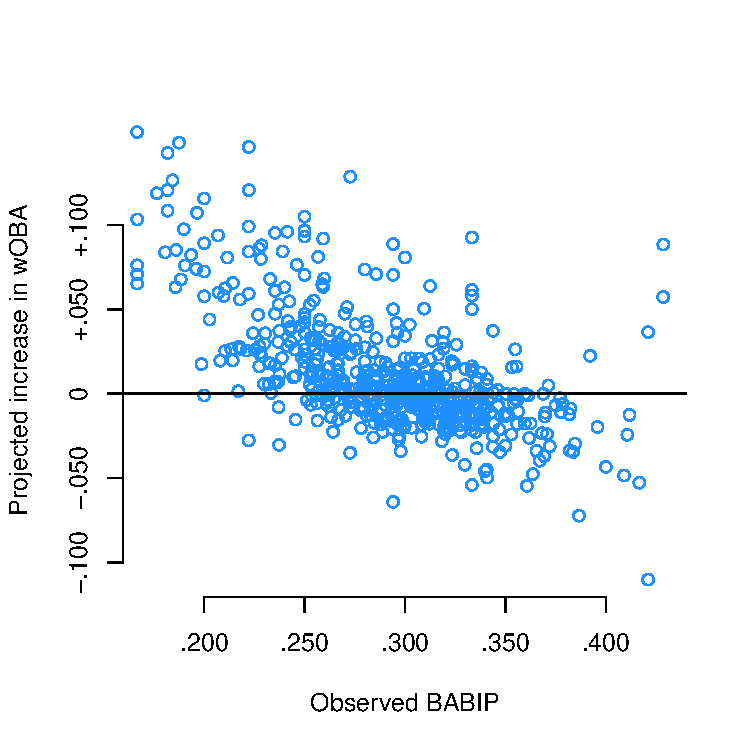
\includegraphics[width = 0.7\textwidth]{../figs/woba-v-babip-slides.pdf}
\end{frame}

\begin{frame}
\centering\LARGE Estimator Comparison
\end{frame}

\begin{frame}{Test RMSE for different talent estimators}
Randomly split PAs into training and test sets, using training set to predict
test set rate for each outcome\\~\\
\centering
\begin{tabular}{c|cccc}
    & Naive & Regressed & Ridge & Random\\
    \hline
G   & 4.41  & 3.98      & 3.97  & 3.98\\
F   & 4.45  & 3.97      & 3.99  & 3.98\\
K   & 4.25  & 3.89      & 3.90  & 3.90\\
BB  & 2.60  & 2.38      & 2.39  & 2.39\\
HBP & 1.04  & 0.89      & 0.88  & 0.88\\
1B  & 3.66  & 3.09      & 3.08  & 3.08\\
2B  & 2.21  & 1.68      & 1.67  & 1.67\\
3B  & 0.82  & 0.63      & 0.64  & 0.64\\
HR  & 1.71  & 1.52      & 1.51  & 1.50
\end{tabular}\\
{\scriptsize Units: percentage points}\\
{\bf Upshot}: In this simple example, these three estimators are virtually
equivalent!
\end{frame}

\begin{frame}{Ridge estimator vs. Regressed estimator for 1B rate}
\centering
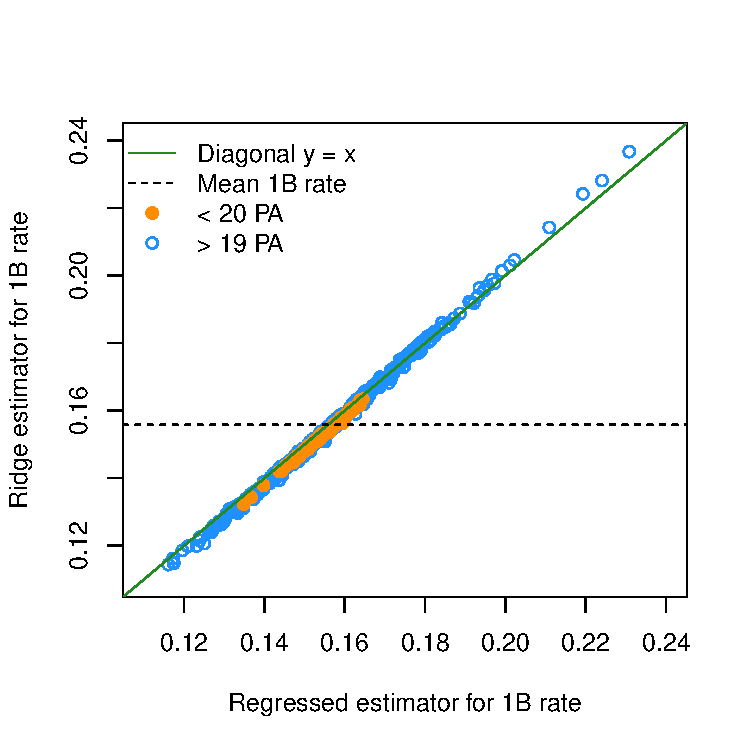
\includegraphics[width = 0.7\textwidth]{../figs/regul-as-regre-c.pdf}
\end{frame}

\begin{frame}
\centering\LARGE True wOBA Validation
\end{frame}

\begin{frame}{Validation}
\begin{itemize}
\item Evaluate results on 2015 MLB regular season PAs
\begin{itemize}
    \item Discard intentional walks, catcher interferences
    \item Discard PAs in which pitcher is batting
\end{itemize}
\item Fit each method on training set to predict wOBA in test set
\begin{itemize}
    \item $\{O_i = 0\} \Rightarrow$ training set with prob. 90\%
    \item $\{O_i = 1\} \Rightarrow$ test set with prob. 90\%
\end{itemize}
\item Training set: 93,868 PAs
\item Test set: 82,692 PAs
\end{itemize}
\begin{center}
\begin{tabular}{c|cccc}
Estimator           &  Naive    & Regressed & True          & Mixed\\
\hline
Estimated MSE      & 45.6   & 22.0   & {\bf 17.3} & 18.0\\
Stadard error       &$\pm$4.4&$\pm$1.8&$\pm$1.4 &$\pm$1.5
\end{tabular}\\
{\scriptsize Units: wOBA points}
\end{center}
\end{frame}

\begin{frame}
\centering\LARGE True wOBA Results
\end{frame}

\begin{frame}{True wOBA vs. observed wOBA}
\centering
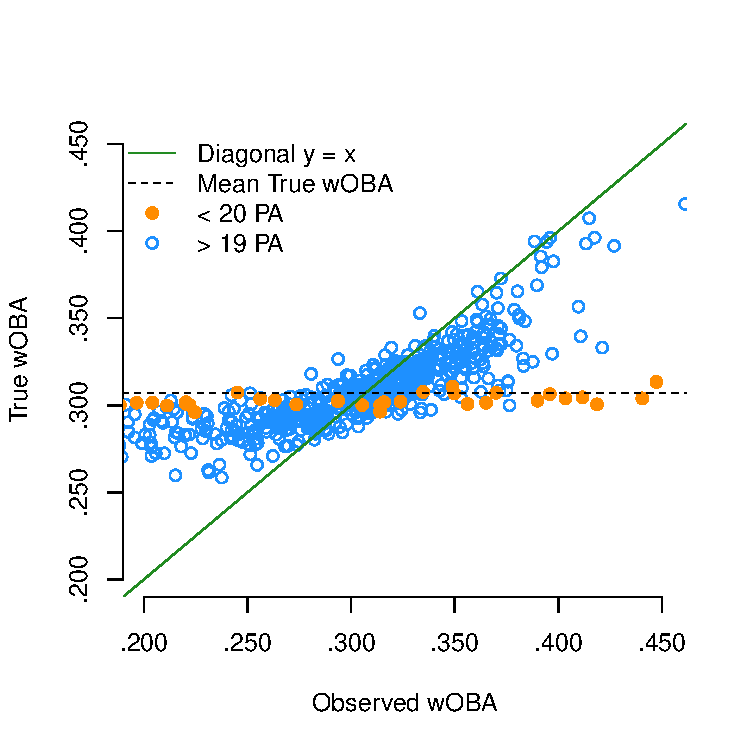
\includegraphics[width = 0.7\textwidth]{../figs/true-woba-batters.pdf}
\end{frame}

\begin{frame}{True wOBA against vs. observed wOBA against}
\centering
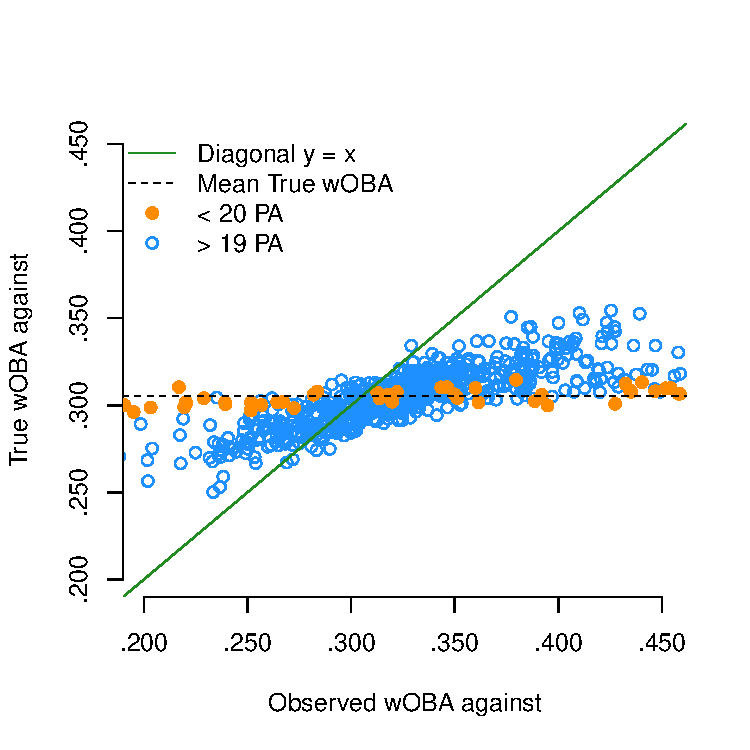
\includegraphics[width = 0.7\textwidth]{../figs/true-woba-pitchers.pdf}
\end{frame}

\begin{frame}{Top 5 and bottom 5 batters by True wOBA}
\centering
\scriptsize
\hspace*{-1cm}
\begin{tabular}{c|ccc}
      &Batter        &Team& True wOBA \\
\hline
      &Bryce Harper     &WSN & .416 \\
Top   &Mike Trout       &LAA & .407 \\
5     &Jos\'{e} Bautista&TOR & .399 \\
      &Paul Goldschmidt &ARI & .395 \\
      &Joey Votto       &CIN & .393 \\
      &...              &    &      \\*
      &Alexi Amarista   &SDP & .270 \\
Bottom&Chris Owings     &ARI & .269 \\
5     &Ren\'{e} Rivera  &TBR & .265 \\
      &Danny Santana    &MIN & .265 \\
      &Omar Infante     &KCR & .262 
\end{tabular}
\end{frame}

\begin{frame}{Top 5 and bottom 5 pitchers by True wOBA against}
\centering
\scriptsize
\hspace*{-1cm}
\begin{tabular}{c|ccc}
      & Pitcher    &Team& True wOBA against\\
\hline
      &Jake Arrieta   &CHC & .255 \\
Top   &Clayton Kershaw&LAD & .256 \\
5     &Zack Greinke   &LAD & .261 \\
      &Wade Davis     &KCR & .267 \\
      &Dallas Keuchel &HOU & .267 \\
      &...            &    &      \\
      &Jeremy Guthrie &KCR & .346 \\
Bottom&Matt Boyd      &DET & .346 \\
5     &David Holmberg &CIN & .349 \\
      &Dustin McGowan &PHI & .354 \\
      &Allen Webster  &ARI & .356
\end{tabular}
\end{frame}

\begin{frame}{Top differences between naive and True wOBA}
\centering
\scriptsize
\hspace*{-0.5cm}
\begin{tabular}{c|ccc}
      &Batter      &Team& $\Delta$wOBA\\
\hline
      &Wilson Ramos    &WSN & +.022\\
Top   &Michael Taylor  &WSN & +.021\\
5     &Albert Pujols   &LAA & +.017\\
      &Alcides Escobar &KCR & +.016\\
      &Chris Owings    &ARI & +.014\\
      & ...            &    &      \\
      &Anthony Rizzo   &CHC &--.035\\
Bottom&Nolan Arenado   &COL &--.037\\
5     &Charlie Blackmon&COL &--.039\\
      &Bryce Harper    &WSN &--.045\\
      &David Peralta   &ARI &--.046
\end{tabular}
\\
\vspace{5mm}
Min. 500 PA
\end{frame}

\begin{frame}{Top differences between naive and True wOBA against}
\centering
\scriptsize
\hspace*{-0.5cm}
\begin{tabular}{c|ccc}
      &Pitcher     &Team&$\Delta$wOBA against\\
\hline
      &Chris Rusin    &COL &--.068\\
Top   &Kyle Kendrick  &COL &--.062\\
5     &Jerome Williams&PHI &--.047\\
      &Matt Garza     &MIL &--.045\\
      &Kyle Lohse     &MIL &--.041\\
      &...            &    &      \\
      &Jacob deGrom   &NYM & +.016\\
Bottom&Sonny Gray     &OAK & +.016\\
5     &Clayton Kershaw&LAD & +.019\\
      &Jake Arrieta   &CHC & +.021\\
      &Zack Greinke   &LAD & +.023
\end{tabular}
\\
\vspace{5mm}
Min. 500 PA
\end{frame}

\begin{frame}{Discussion}
Three contributions:
\begin{itemize}
\item We remind everyone of regression to the mean for interpretation of small
    sample sizes
\item We explain relationship between regularized linear models and regression
    to the mean
\item We compare regularized linear models with linear mixed effects models
\end{itemize}
\end{frame}

\begin{frame}{Thank you!}
\centering
\Huge Questions?\\~\\
\normalsize
Scott Powers            \hfill  Eli Shayer\\
sspowers@stanford.edu   \hfill  eshayer@stanford.edu\\
                        \hfill  elishayer.com\\~\\
{\tt github.com/sspowers/true-woba}\\~\\
{\tt stanfordsportsanalytics.com}\\
\hfill
\includegraphics[width = 1in]{../figs/ssac.png}
\end{frame}

\end{document}
